\documentclass[journal]{IEEEtran}
\usepackage{graphicx}
\usepackage{subcaption}

\ifCLASSINFOpdf
\else
\fi

\hyphenation{op-tical net-works semi-conduc-tor}

\begin{document}


\title{Spectral Weighting and Spatial Biasing\\ for Hyperspectral K-Means Clustering}


\author{Daniel Hanson, Sam Kreter, Brendan Marsh, and Christina R.S. Mosnick}

\markboth{ECE/CS 4720 (Spring 2016): Introduction to Machine Learning and Pattern Recognition}
{Shell \MakeLowercase{\textit{et al.}}: Bare Demo of IEEEtran.cls for IEEE Journals}

\maketitle

\begin{abstract}
Here we present an approach to unsupervised clustering of hyperspectral imaging data, specifically the Indian Pines data set. A baseline approach of simple k-Means on the raw hyperspectral data is used to compare successive iterations of our final approach, which utilizes a high level dimensionality reduction via band selection, feature weighting, and k-Means clustering combined with a spatial biasing algorithm. The final algorithm achieved a Rand index of 88.6\% when compared to the Indian Pines ground truth. A major conclusion that can be drawn from the study is that commonly used methods in dimensionality reduction and unsupervised clustering, like principal component analysis and density-based spatial clustering of applications with noise, are not always necessary for robust clustering, and in this case performed poorly compared to our simpler approach.
\end{abstract}

\begin{IEEEkeywords}
    Principal Component Analysis (PCA), k-Means, Normalization, Whitening, Spectral Imaging.
\end{IEEEkeywords}

\IEEEpeerreviewmaketitle

\section{Introduction}

\IEEEPARstart{U}{nsupervised} clustering methods have applications in many fields, such as marketing, city planning, and insurance. For example, mass amounts of consumer data can be aggregated and clustered to gain insights into customer behaviors and trends \cite{ClusterTutorial}. City planners can use clustering to identify groups of housing based on house type, value, and geographical location \cite{ClusterTutorial}. Property and casualty insurers can analyze variables related to staged car accidents resulting in fraudulent insurance claims. Some of these variables are low vehicle value, average number of visits to the chiropractor, and absence of a police report \cite{FraudAnalysis}. The challenge this report attempts to address is distinguishing distinctive fields from a spatial image consisting of multiple spectral bands.\\

The Indian Pines \cite{IndianPines} dataset used in our research consisted of two-hundred wavelength bands, and was taken over a landscape of sixteen different field types such as alfalfa, grass, grass-mowed, corn, etc. As an example of the challenges present in satellite image processing, viewing a standard red, green, blue image of the fields from above may not give enough useful information to differentiate between fields such as grass and mowed grass. Using a hyperspectral sensor, on the other hand, can provide a vastly larger amount of data, as well as many different types of data, by collecting more wavelengths than are visible to the human eye. Certain wavelengths (such as infrared) by themselves can provide useful information, as well as unique combinations of many bands. By contrast, some wavelengths contain no useful identifying information whatsoever. The challenge lies in implementing a suitable unsupervised clustering method to parse through the spectral bands to find significant clusters representing fields.\\

%\hfill mds

%\hfill August 26, 20154

\section{Implementation}
  \subsection{K-Means \& PCA Implementation}
    In order to efficiently implement a variety of candidate algorithms for this unsupervised clustering problem, we decided to use the popular python machine learning library scikit-learn \cite{ScikitLearnAPI}.\\

    We first decided to implement the k-Means algorithm as a baseline test. Given that we knew in advance the number of classes we needed to find, the task naively lent itself nicely to a k-Means clustering approach. We used the scikit-learn's k-Means \cite{ScikitLearnAPI} implementation because it allows for a good amount of fine tuning through its many parameter options.\\

    We next looked into dimensionality reduction options. The initial dataset is 145x145 pixels in size with 220 spectral layers for each pixel. We again used scikit-learn to implement Principal Component Analysis, or PCA. This implementation also allows for whitening to normalize, which can be used as another parameter during the experiments to find the best method.\\

    \begin{figure}[h!]
      \centering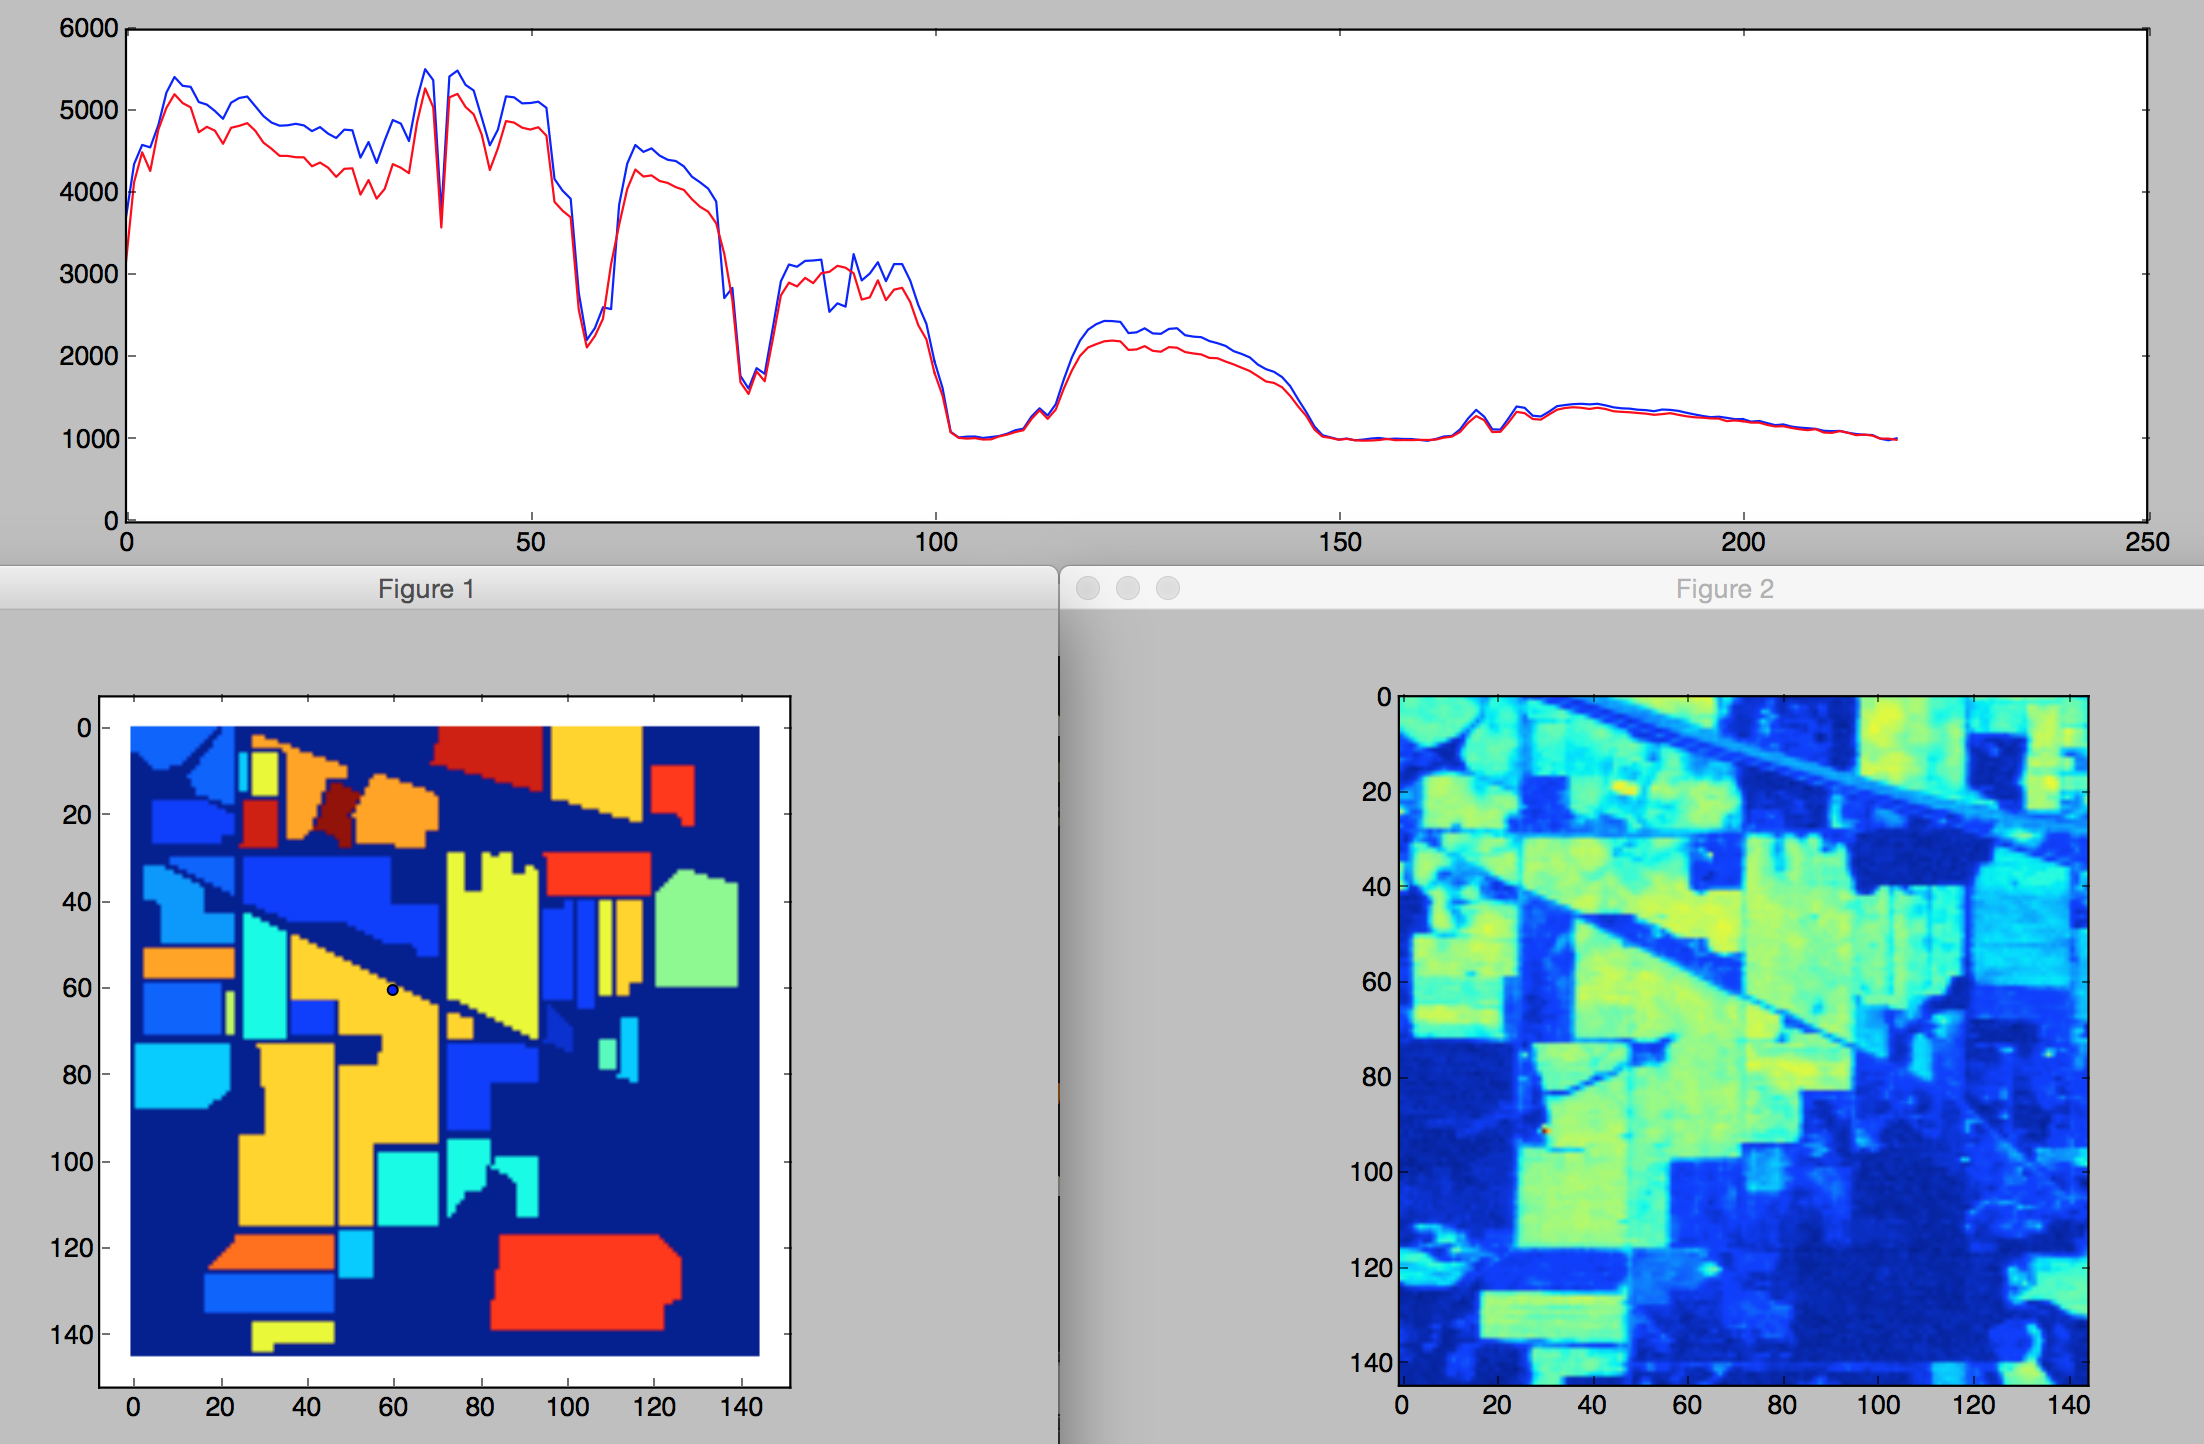
\includegraphics[width=\columnwidth]{images/tool.png}
      \caption{Spectral Data Viewer}
      \label{fig:Viewer}
    \end{figure}

    In order to gain a better understanding of the data, we developed a simple tool using python and matplotlib to visualize each layer of the spectral data. Figure \ref{fig:Viewer} shows the simple interface. After selecting an X, Y spatial position and a spectral layer number, the top graph shows the relationship between the currently selected pixel’s spectral data (in blue) and the previously visited pixel’s data (in red). The bottom-right graph shows the visual representation of the specified spectral layer. This allows us to easily see each layer’s impact on the final clustering of the data. The bottom-left graph shows the final ground truth of the dataset for reference, along with a black point indicating the current X, Y position.\\

    Using this tool, we were able to create a normalization function to weight the more distinctive spectral layers more heavily, as shown in Figure \ref{fig:GoodLayer}, while assigning a smaller weight to the less indicative layers such as shown in Figure \ref{fig:BadLayer}.\\


    \begin{figure}[h!]
      \centering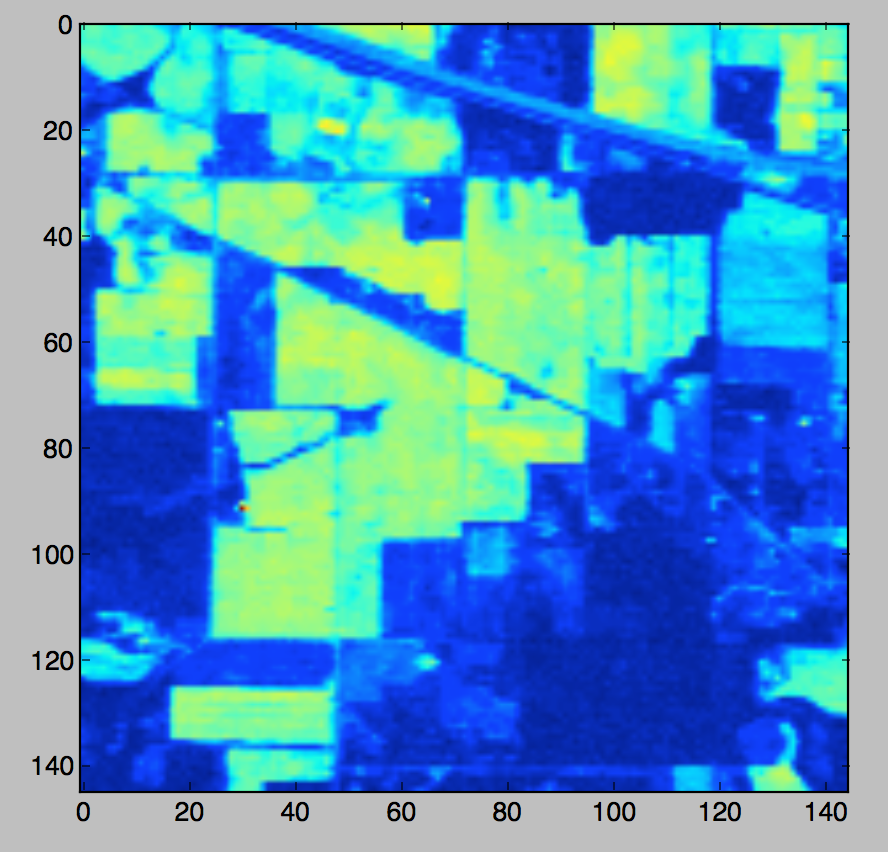
\includegraphics[width=6cm]{images/allStarSpec.png}
      \caption{Useful Spectral Layer}
      \label{fig:GoodLayer}
    \end{figure}

    \begin{figure}[h!]
      \centering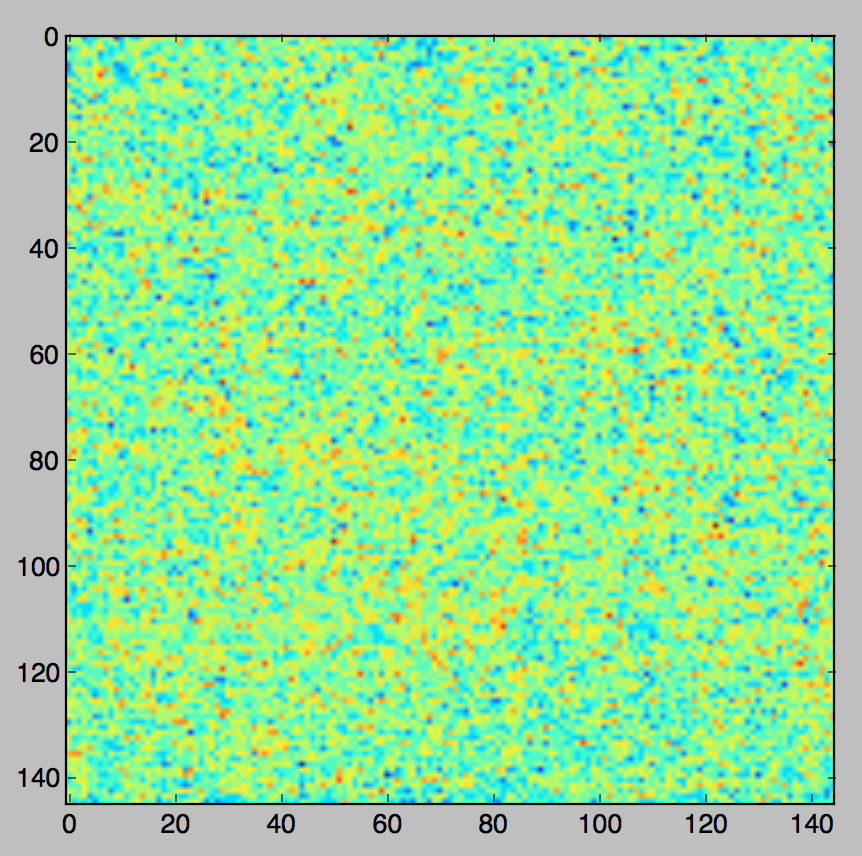
\includegraphics[width=6cm]{images/horribleSpec.png}
      \caption{Useless Spectral Layer}
      \label{fig:BadLayer}
    \end{figure}

    After applying normalization on the spectral layers, we experimented with giving a pixel’s spatial coordinates greater impact in the final clusterings. Because the initial data processing converted the data cube into a set of feature vectors, spatial information was lost. To fix this, we append the X and Y position onto the spectral feature vector and factored the X and Y weights into the normalization.\\

  \subsection{Neighborhood Implementation}
    Observation of the data revealed that neighboring pixels are very often in the same class; it seems intuitive that spatially close areas have similar spectral signatures.  This observation can be used to enforce a bias on any proposed clustering provided by k-Means or any other clustering algorithm. The neighborhood biasing algorithm we created iterated through each pixel, surveying its neighbors within a defined spatial radius, and found the mode of the classes found. If a certain class was found to be very predominant in the immediate spatial neighborhood, the class of the current pixel was changed to that class. The algorithm is iterative and can be run as many times as desired until convergence. The goal of the neighborhood bias algorithm was the removal of spectral outliers in otherwise well-defined clusters and an overall smoothing of the output provided by some clustering algorithms. This approach can be beneficial if there are many spectrally noisy outliers, but could also be bad if there are small clusters that could be smoothed over by the algorithm. The radius of the polling neighborhood and the number iterations can control the level of smoothing. In our case, we generally used a small radius of 2 pixels and 10 iterations of the algorithm.\\

    \begin{figure}[h!]
      \centering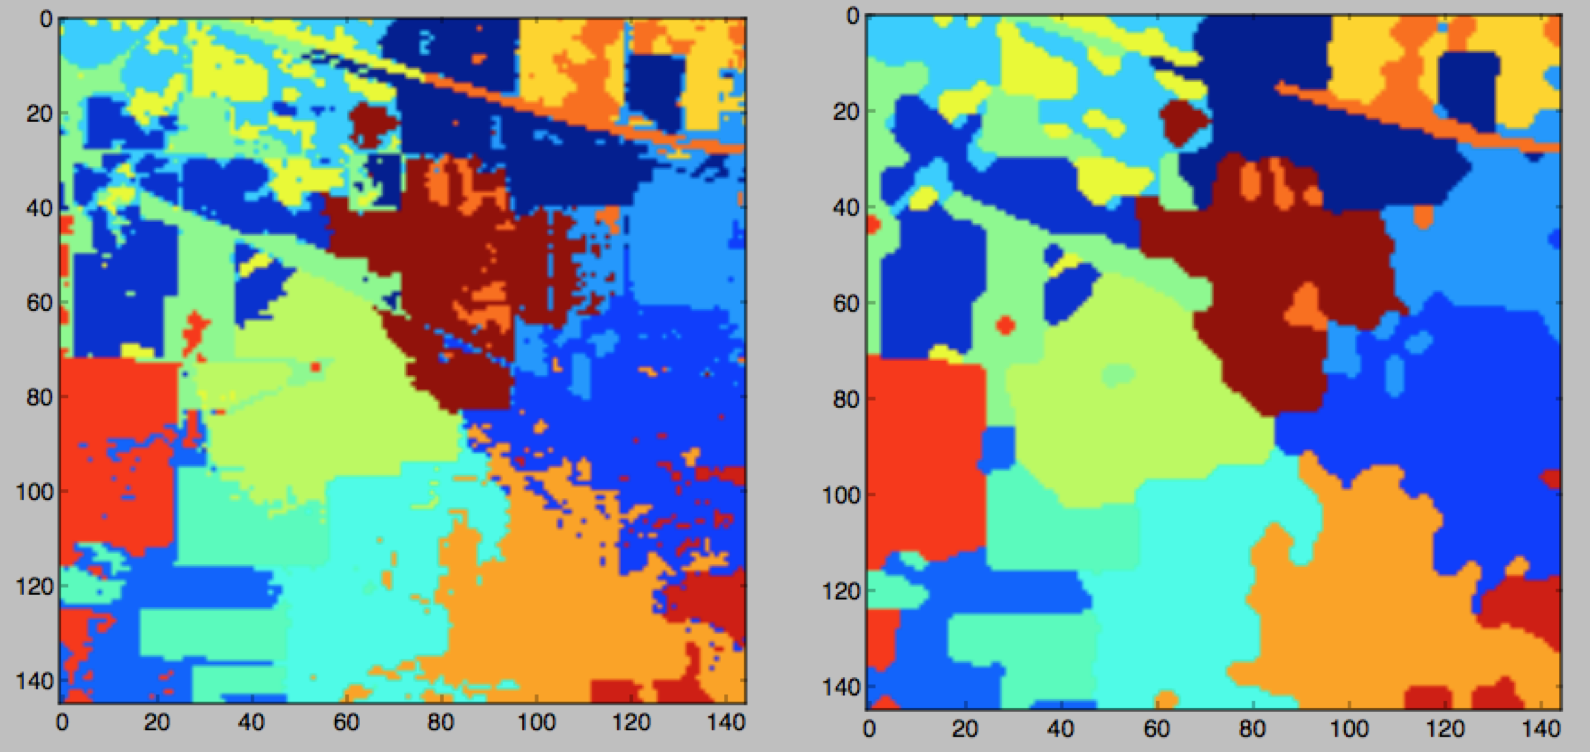
\includegraphics[width=\columnwidth]{images/BandUnB.png}
      \caption{Before and After Neighborhood Bias}
      \label{fig:NeighborhoodBias}
    \end{figure}

\section{Experiments}
  In order to find the best approach, we used a baseline implementation of k-Means with 16 cluster centers. We also used both the Rand index and the adjusted Rand index as a quantitative measurement of accuracy; the adjusted Rand index arguably provides a more robust metric of classification accuracy as it accounts for the random chance of correct classification in a way that the Rand index does not. An increase in the number of possible clusters can lead to an artificially inflated Rand index.\\

  There are a number of parameters in our implementation to optimize, including normalized weighting of the bands, the use of PCA (or not), and whitening.  In order to have a homogeneous computing environment for long running jobs, we set up a server using Amazon Web Services \cite{AWS}. We then ran a script to run the algorithm with different permutations of parameters in order to optimize the Rand index. Figure \ref{fig:Parameters} shows the different parameters at play and their classification accuracy.\\

  The weighting of the spatial data, defined as a pixel’s row and column in the image, optimized the accuracy with weights of 2 times the original values. The overall spectral weighting gave maximum accuracy with a weight of .001. These weights roughly correspond to equally weighing the magnitude of the spatial and spectral features. The experiment also showed that the spectral layers 167, 52, and 120 made the most impact on the final clusters when weighted at 2, .1, and .1 respectively. Although bands 52 and 120 were reduced, they still had a weight of 10x higher than the other spectral bands reduced to .001. We also found that using PCA had a negative effect on the final result as compared to simple band selection. There are a number of reasons why PCA may not perform well in this context; PCA picks out features which contain the most variance, but variance does not necessarily correspond to usefulness. In our case, the features extracted by PCA contained almost all of the variance in a single feature vector, and much of the useful, distinctive data was lost.\\

  \begin{figure}[h!]
    \centering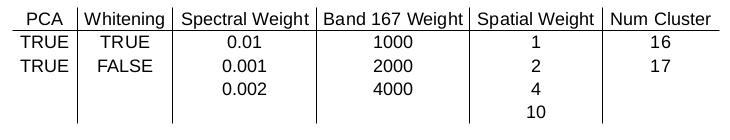
\includegraphics[width=\columnwidth]{images/parameters.png}
    \caption{Parameters for Experiments}
    \label{fig:Parameters}
  \end{figure}

  The parameter set discussed above produced a Rand index of 0.883907 and an adjusted Rand index of 0.095498. This was a great improvement on the baseline k-Means algorithm of 0.820231 for the Rand index and for 0.034969 the adjusted Rand index.\\

  After applying the neighborhood biasing algorithm, the Rand index increased to 0.886272 and the adjusted Rand index increased to 0.100829, which is also significantly better than the baseline values 0.820231 and 0.034969 and the scores produced by the same approach without neighborhood biasing.\\

  From these experiments we were able to see the different trends in the parameter sets. The first trend was in the normalization set. The x and y position had a maximum effect at a weight of 2 times the original. The overall spectral weighting was best at .001 times to make it comparable to the positional. The experiment also shows that the spectral layers 167, 52, and 120 give the best impact on the final clusters weighted at 2000, 100, 100 respectively. We also found that using PCA had a negative effect on the final clustering result since the PCA would form the spectral clusters together based off their variance not saving the spatial representation.\\

  This set of parameters produced a rand index of 0.883907 and a adjusted rand index of 0.095498 which is a great improvement on the baseline K-Means algorithm of 0.820231 for the rand index and for 0.034969 the adjusted rand index.\\

  In order to test the neighborhood bias algorithm, we simply used the rand index and adjusted rand index to compare with out baseline and other algorithms. The algorithm came up with .886272 for the rand and 0.100829 for the adjusted rand index which is also significantly better than the baseline of 0.820231and 0.034969 respectively.\\

\section{Conclusion}
  The Indian pines hyperspectral data was clustered to produce a Rand index of 0.886 as compared to the ground truth via our method combining band selection for dimensionality reduction, feature weighting, k-Means clustering, and a new algorithm based spatial biasing. The development of this method grew out of a baseline implementation using just a k-Means clustering, and through the iterations of the approach some key insights were made. Primarily, we found that PCA does not perform well in some cases compared to the simpler method of selecting individual wavelengths for dimensionality reduction. Furthermore, more complex clustering methods like DBSCAN were found to perform more poorly as compared to simple k-Means. This, of course, is not a general result as k-Means can often perform very poorly. However, this approach demonstrates that simpler clustering methods can still be superior depending on the data set. Finally, a spatial biasing algorithm was developed that modifies any arbitrary clustering output to account for the a pixels relationship with its spatial neighbors. In almost all cases, this biasing provided a modest gain in terms of the Rand and adjusted Rand index, and provided qualitatively better results that excluded spectral outliers.\\


\ifCLASSOPTIONcaptionsoff
  \newpage
\fi

\begin{thebibliography}{1}

\bibitem{AWS}
  Amazon. \emph{Amazon Web Services.} https://aws.amazon.com/. N.p., 2016. Web. 4 May 2016.

\bibitem{BishopBook}
  Bishop, Christopher M. \emph{Pattern Recognition And Machine Learning.} New York: Springer, 2006. Print.

\bibitem{Blondel}
  Blondel, Mathieu. \emph{Fuzzy K-means and K-medians.} https://gist.github.com/mblondel/1451300. N.p., 2011. Web. 4 May 2016.

\bibitem{ScikitLearnAPI}
  Buitinck et al., \emph{API design for machine learning software: experiences from the scikit-learn project.} ECML PKDD Workshop, pp. 108-122, 2013.

\bibitem{FraudAnalysis}
  Francis, Louise. \emph{Applications of Unsupervised Learning in Property and Casualty Insurance with Emphasis on Fraud Analysis} http://www.slideshare.net/salfordsystems/final-applications-of-unsupervised-learning-in-pc. N.p., 2012. Web. 4 May 2016.

\bibitem{ClusterTutorial}
  Matteo, Matteucci. \emph{A Tutorial on Clustering Algorithms.} http://home.deib.polimi.it/matteucc/Clustering/tutorial\_html/. N.p., 2016. Web. 4 May 2016.

\bibitem{IndianPines}
  Purdue Research Foundation. \emph{Hyperspectral Remote Sensing Scenes.} http://www.ehu.eus/ccwintco/index.php?title=Hyperspectral \_Remote\_Sensing\_Scenes. N.p., 2016. Web. 4 May 2016.

\bibitem{DataMining}
  Zhang, Hantao. \emph{Unsupervised Learning.} http://homepage.cs.uiowa.edu/\~hzhang/c145/notes/chap18b.pdf. N.p., 2016. Web. 4 May 2016.

\end{thebibliography}

\end{document}